\documentclass[tikz]{standalone}
\usepackage{tikz}
    \usetikzlibrary{positioning}

\tikzset{basic/.style={draw,fill=blue!20,text width=1em,text badly centered}}
\tikzset{input/.style={basic,circle,fill=red!30}}
\tikzset{weights/.style={basic,rectangle}}
\tikzset{sum/.style={basic,circle,fill=green!30}}
\tikzset{functions/.style={basic,circle,fill=blue!30}}


\begin{document}
    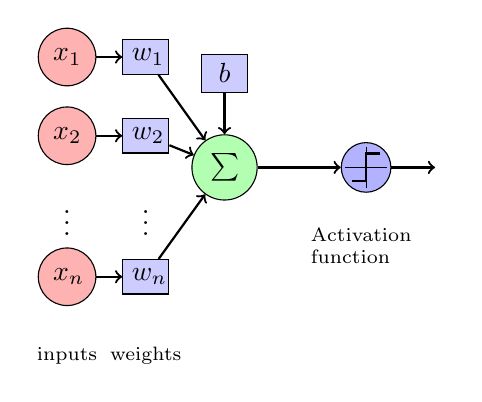
\begin{tikzpicture}
        \node[functions] (center) {};
        \node[below of=center,font=\scriptsize,text width=4em] {Activation function};
        \draw[thick] (0.5em,0.5em) -- (0,0.5em) -- (0,-0.5em) -- (-0.5em,-0.5em);
        \draw (0em,0.75em) -- (0em,-0.75em);
        \draw (0.75em,0em) -- (-0.75em,0em);
        \node[right of=center] (right) {};
            \path[draw,thick,->] (center) -- (right);
        \node[sum,left=3em of center] (left) {$\sum$};
            \path[draw,thick,->] (left) -- (center);
        \coordinate[left of=left] (input);
        \node[weights,above =0.5em of input] (2) {$w_2$} -- (2) node[input,left of=2] (l2) {$x_2$};
            \path[draw,thick,->] (l2) -- (2);
            \path[draw,thick,->] (2) -- (left);
        \node[below of=2] (dots) {$\vdots$} -- (dots) node[left of=dots] (ldots) {$\vdots$};
        \node[weights,below = 0.5em of dots] (n) {$w_n$} -- (n) node[input,left of=n] (ln) {$x_n$};
            \path[draw,thick,->] (ln) -- (n);
            \path[draw,thick,->] (n) -- (left);
        \node[weights,above of=2] (1) {$w_1$} -- (1) node[input,left of=1] (l1) {$x_1$};
            \path[draw,thick,->] (l1) -- (1);
            \path[draw,thick,->] (1) -- (left);
        \node[weights,above = 1.5em of left] (0) {$b$};
            \path[draw,thick,->] (0) -- (left);
        \node[below of=ln,font=\scriptsize] {inputs};
        \node[below of=n,font=\scriptsize] {weights};
    \end{tikzpicture}
\end{document}